% === T10 - Álgebra de Boole y Compuertas ===
% David Alejandro Gonzalez Marquez
% fokerman@gmail.com
% https://github.com/fokerman/computingSystemsCourse

\RequirePackage[2020-02-02]{latexrelease}

\documentclass[aspectratio=169]{beamer}
\usepackage{../packages}

\title{\Huge Álgebra de Boole y Compuertas}
\author{David Alejandro González Márquez}
\institute{}

\date{}

\begin{document}

\begin{frame}[plain]
    \titlepage
    \begin{textblock}{100}(30,80)
    \begin{tcolorbox}[size=small,width=\textwidth,colback={gray!30},title={}]
    \begin{center}
     \scriptsize Clase disponible en: \url{https://github.com/fokerman/computingSystemsCourse}
    \end{center}
    \end{tcolorbox}
    \end{textblock}
%     \begin{textblock}{140}(10,70)
%     \textcolor{rojo}{
%     \textbf{Atención}: La clase será grabada por el anfitrión para su posterior y eventual uso académico dentro de nuestra institución. Su participación en la clase implica brindar su consentimiento para participar en la grabación, aunque pueden mantener su video apagado.}
%     \end{textblock}
\end{frame}

\begin{frame}[fragile]
    \frametitle{Álgebra de Boole}
    Las computadoras operan de forma digital, con circuitos que pueden tomar \textbf{dos estados}:\\
    \begin{center}
    \textit{verdadero} (1) y \textit{falso} (0).\\ 
    \end{center}
    \bigskip
    Para describir el funcionamiento de estos circuitos, vamos a necesitar un nuevo tipo de álgebra.\\
    \bigskip
    \pause
    \begin{block}{\textbf{Álgebra de Boole} {\small- George Boole (1815-1864)}}
    Sistema algebraico para el estudio sistemático de la lógica proposicional, 
    donde las variables y funciones pueden adoptar dos estados.
    Resulta una formalización apropiada para representar información digital y permite expresar las operaciones que realizan los circuitos digitales.
    \end{block}    
\end{frame}

\begin{frame}[fragile]
    \frametitle{Álgebra de Boole}
    \begin{block}{Función Booleana}
    Toma una o más variables de entrada y produce un resultado que depende solo de los valores de entrada.
    Las variables pueden tener solo dos estados \texttt{0} (falso) o \texttt{1} (verdadero).
    \end{block}
    \pause
    Con $n$ entradas, las funciones booleanas tienen $2^n$ combinaciones posibles para sus entradas.\\
    \bigskip
    \textcolor{gray}{Ejemplo}\\
    Para $f(A,B)$ las posibles entradas son: \texttt{$f(0,0)$}, \texttt{$f(0,1)$}, \texttt{$f(1,0)$} y \texttt{$f(1,1)$}.\\
%     \texttt{$(A=0,B=0)$}, \texttt{$(A=0,B=1)$}, \texttt{$(A=1,B=0)$} y \texttt{$(A=1,B=1)$}\\
    \bigskip
    \textbf{Tabla de verdad}\\ Describe todas las posibles combinaciones de entradas y resultados para una función booleana.
\end{frame}

\begin{frame}[fragile,t]
    \frametitle{Álgebra de Boole - Operadores}
    Tenemos tres operaciones básicas dentro del Álgebra de Boole.\\
    \begin{textblock}{45}(7.5,18)
    \begin{block}{\texttt{NOT} $\rightarrow$ \Large \textcolor{naranjauca}{ $\overline{\texttt{A}}$ }}
     Invierte el valor de entrada de \texttt{1} a \texttt{0} y viceversa.
    \vspace{0.98cm} % FIX SIZE
    \begin{center}
    \begin{tabular}{c|c}
    \texttt{A} & \texttt{NOT} \\
    \hline
    \texttt{0} & \texttt{1} \\
    \texttt{1} & \texttt{0} \\
    \end{tabular}
    \end{center}
    \vspace{0.28cm} % FIX SIZE
    \end{block}
    \end{textblock}    
    \begin{textblock}{45}(57.5,18)
    \begin{block}{\texttt{AND} $\rightarrow$ \Large \textcolor{naranjauca}{ $\texttt{A}\cdot\texttt{B}$ }}
    Verdadero (\texttt{1}) si y solo si ambas entradas son verdaderas. %\wedge
    \begin{center}
    \begin{tabular}{cc|c}
    \texttt{A} & \texttt{B} & \texttt{AND} \\
    \hline
    \texttt{0} & \texttt{0} & \texttt{0} \\
    \texttt{0} & \texttt{1} & \texttt{0} \\
    \texttt{1} & \texttt{0} & \texttt{0} \\
    \texttt{1} & \texttt{1} & \texttt{1} \\
    \end{tabular}
    \end{center}
    \end{block}
    \vspace{0cm} % FIX SIZE
    \end{textblock}
    \begin{textblock}{45}(107.5,18)
    \begin{block}{\texttt{OR} $\rightarrow$ \Large \textcolor{naranjauca}{ $\texttt{A}+\texttt{B}$ }}
    Verdadero (\texttt{1}) si al menos una entrada es verdadera. % \vee
    \vspace{0.45cm} % FIX SIZE
    \begin{center}
    \begin{tabular}{cc|c}
    \texttt{A} & \texttt{B} & \texttt{OR} \\
    \hline
    \texttt{0} & \texttt{0} & \texttt{0} \\
    \texttt{0} & \texttt{1} & \texttt{1} \\
    \texttt{1} & \texttt{0} & \texttt{1} \\
    \texttt{1} & \texttt{1} & \texttt{1} \\
    \end{tabular}
    \end{center}
    \end{block}
    \end{textblock}
\end{frame}

\begin{frame}[fragile,t]
    \frametitle{Álgebra de Boole - Ejemplo}
%     \begin{block}{\small Operadores}
%      \small \texttt{NOT} ($\overline{x}$): Invierte el valor de entrada de \texttt{1} a \texttt{0} y viceversa.\\
%      \small \texttt{AND} ($x \cdot y$): Verdadero (\texttt{1}) si y solo si ambas entradas son verdadero.\\ %\wedge
%      \small \texttt{OR } ($x + y$): Verdadero (\texttt{1}) si al menos una entrada es verdadero. % \vee
%     \end{block}
    \begin{textblock}{16}(68,5)
    \begin{block}{\texttt{NOT}}
    \begin{tabular}{c|c}
    \texttt{A} & \textcolor{naranjauca}{ $\overline{\texttt{A}}$} \\
    \hline
    \texttt{0} & \texttt{1} \\
    \texttt{1} & \texttt{0} \\
    \end{tabular}
    \end{block}
    \end{textblock}
    \begin{textblock}{24}(90,5)
    \begin{block}{\texttt{AND}}
    \begin{tabular}{cc|c}
    \texttt{A} & \texttt{B} & \textcolor{naranjauca}{ $\texttt{A}\cdot\texttt{B}$} \\
    \hline
    \texttt{0} & \texttt{0} & \texttt{0} \\
    \texttt{0} & \texttt{1} & \texttt{0} \\
    \texttt{1} & \texttt{0} & \texttt{0} \\
    \texttt{1} & \texttt{1} & \texttt{1} \\
    \end{tabular}
    \end{block}
    \end{textblock}
    \begin{textblock}{25}(120,5)
    \begin{block}{\texttt{OR}}
    \begin{tabular}{cc|c}
    \texttt{A} & \texttt{B} & \textcolor{naranjauca}{ $\texttt{A}+\texttt{B}$} \\
    \hline
    \texttt{0} & \texttt{0} & \texttt{0} \\
    \texttt{0} & \texttt{1} & \texttt{1} \\
    \texttt{1} & \texttt{0} & \texttt{1} \\
    \texttt{1} & \texttt{1} & \texttt{1} \\
    \end{tabular}
    \end{block}
    \end{textblock}
    \vspace{2cm}
    \textcolor{gray}{Ejemplo:}\\
    $f(A,B)$ $=$ $(A \cdot B) + (\overline{A} \cdot \overline{B})$\\
    \bigskip
    {\textbf{Tabla de verdad}}
    \begin{center}
    \begin{tabular}{cc|l|c}
    \texttt{A} & \texttt{B} & $(A \cdot B) + (\overline{A} \cdot \overline{B})$ & $f$ \\
    \hline
    \texttt{0} & \texttt{0} &
    \uncover<2->{$(0 \cdot 0) + (\overline{0} \cdot \overline{0})$ $\rightarrow$} \uncover<3->{$(0 \cdot 0) + (1 \cdot 1)$ $\rightarrow$} \uncover<4->{$0 + 1$} & \uncover<4->{\texttt{1}} \\
    \texttt{0} & \texttt{1} &
    \uncover<5->{$(0 \cdot 1) + (\overline{0} \cdot \overline{1})$ $\rightarrow$ $(0 \cdot 1) + (1 \cdot 0)$ $\rightarrow$ $0 + 0$} & \uncover<5->{\texttt{0}} \\
    \texttt{1} & \texttt{0} &
    \uncover<5->{$(1 \cdot 0) + (\overline{1} \cdot \overline{0})$ $\rightarrow$ $(1 \cdot 0) + (0 \cdot 1)$ $\rightarrow$ $0 + 0$} & \uncover<5->{\texttt{0}} \\
    \texttt{1} & \texttt{1} &
    \uncover<5->{$(1 \cdot 1) + (\overline{1} \cdot \overline{1})$ $\rightarrow$ $(1 \cdot 1) + (0 \cdot 0)$ $\rightarrow$ $1 + 0$} & \uncover<5->{\texttt{1}} \\
    \end{tabular}
    \end{center}
\end{frame}

\begin{frame}[fragile]
    \frametitle{Álgebra de Boole}
    Propiedades para las operaciones ($\cdot$) y ($+$)
    \begin{center}
    \renewcommand{\arraystretch}{1.5}
    \begin{tabular}[h]{|c|c|c|} \rowcolor{gray!15}
    \hline
    Identidad       &      $1 \cdot A=A$                             &     $0+A=A$                  \\
    Nulo            &      $0 \cdot A=0$                             &     $1+A=1$                  \\ \rowcolor{gray!15}
    Idempotencia    &      $A \cdot A=A$                             &     $A+A=A$                  \\ 
    Inverso         &      $A \cdot \overline{A}=0$                  &     $A+\overline{A}=1$       \\ \rowcolor{gray!15}     
    Conmutatividad  &      $A \cdot B=B \cdot A$                     &     $A+B=B+A$                \\
    Asociatividad   &      $(A \cdot B) \cdot C=A \cdot (B \cdot C)$ &     $(A+B)+C=A+(B+C)$        \\ \rowcolor{gray!15}
    Distributividad &      $A + B \cdot C = (A+B) \cdot (A+C)$       &     $A \cdot (B+C)=A \cdot B+A \cdot C$        \\
    Absorci\'on     &      $A \cdot (A+B)=A$                         &     $A+A \cdot B = A$              \\ \rowcolor{gray!15}
    De Morgan       & $\overline{A \cdot B} = \overline{A} + \overline{B}$ & $\overline{A+B} = \overline{A} \cdot \overline{B}$ \\
    \hline
    \end{tabular}
    \end{center}
\end{frame}

\begin{frame}
\frametitle{Álgebra de Boole}
    Ejemplo: reducir la siguiente expresión usando propiedades.\\
    \vspace{0.5cm}
    $\overline{( \overline{X} \cdot Y )} \cdot Z + X \cdot \overline{Z} + \overline{(Y + Z)}$ \hspace{0.5cm} \uncover<8->{$\rightarrow$ \hspace{0.5cm} $ X + \overline{Y} $}\\
    \vspace{0.5cm}
    \pause
    Solución: \\
    \vspace{0.5cm}
    \begin{tabular}{ll}
    $ \overline{( \overline{X} \cdot Y )} \cdot Z + X \cdot \overline{Z} + \overline{(Y + Z)} $              & $\longleftarrow$ De Morgan    \\[4pt]\pause
    $ \overline{( \overline{X} \cdot Y )} \cdot Z + X \cdot \overline{Z} + \overline{Y} \cdot \overline{Z} $ & $\longleftarrow$ distributiva \\[4pt]\pause
    $ \overline{( \overline{X} \cdot Y )} \cdot Z + ( X + \overline{Y} ) \cdot \overline{Z}  $                       & $\longleftarrow$ De Morgan    \\[4pt]\pause
    $ ( X + \overline{Y} ) \cdot Z + ( X + \overline{Y} ) \cdot \overline{Z}  $                              & $\longleftarrow$ distributiva \\[4pt]\pause
    $ ( X + \overline{Y} ) \cdot ( Z + \overline{Z} ) $                                                      & $\longleftarrow$ inverso      \\[4pt]\pause
    $ ( X + \overline{Y} ) \cdot 1  $                                                                        & $\longleftarrow$ identidad    \\[4pt]\pause
    $  X + \overline{Y} $
    \end{tabular}
\end{frame}

\begin{frame}[fragile]
    \frametitle{Lógica Digital}
    Las computadoras están construidas mediante \textbf{circuitos electrónicos}.\\
    \bigskip
    Los circuitos operan de forma digital, tal que cada \textbf{cable} puede tomar dos estados posibles:
    \begin{itemize}
     \item \textcolor{naranjauca}{Nivel lógico \texttt{0}} | \textcolor{verdeuca}{apagado} | \textcolor{verdeuca}{ausencia de tensión}
     \item \textcolor{naranjauca}{Nivel lógico \texttt{1}} | \textcolor{verdeuca}{encendido} | \textcolor{verdeuca}{presencia de tensión}
    \end{itemize}
    \bigskip
    Los ladrillos que nos permiten construir circuitos digitales se denominan \textbf{compuertas}.\\
    \bigskip
    Las compuertas se construyen con componentes electrónicos como \textbf{transistores},\\
    la base de toda la computación moderna basada en semiconductores.
\end{frame}

\begin{frame}[fragile,t]
    \frametitle{Compuertas}
    Las compuertas nos permiten hacer operaciones con las señales eléctricas (\texttt{0} y \texttt{1}).\\
    Toman una o dos entradas, y generan una salida.\\
    \bigskip
    Estos son ejemplos de las \textbf{compuertas básicas}, junto a una tabla que describe su comportamiento.
    \bigskip
    \begin{textblock}{16}(8,37)   \begin{center} \includegraphics[scale=0.6]{img/compuertas-layer1.pdf} \end{center} \end{textblock}
    \begin{textblock}{21}(28,37)  \begin{center} \includegraphics[scale=0.6]{img/compuertas-layer2.pdf} \end{center} \end{textblock}
    \begin{textblock}{21}(53,37)  \begin{center} \includegraphics[scale=0.6]{img/compuertas-layer3.pdf} \end{center} \end{textblock}
    \begin{textblock}{21}(77,37)  \begin{center} \includegraphics[scale=0.6]{img/compuertas-layer4.pdf} \end{center} \end{textblock}
    \begin{textblock}{21}(105,37) \begin{center} \includegraphics[scale=0.6]{img/compuertas-layer5.pdf} \end{center} \end{textblock}
    \begin{textblock}{21}(130,37) \begin{center} \includegraphics[scale=0.6]{img/compuertas-layer6.pdf} \end{center} \end{textblock}
    \begin{textblock}{100}(8,50)
    \begin{tabular}{c|c}
    \multicolumn{2}{c}{\textcolor{naranjauca}{ $\overline{\texttt{A}}$ } } \\
    \texttt{A} & \texttt{NOT} \\
    \hline
    \texttt{0} & \texttt{1} \\
    \texttt{1} & \texttt{0} \\
    \end{tabular}
    \end{textblock}
    \begin{textblock}{100}(28,50)
    \begin{tabular}{cc|c}
    \multicolumn{3}{c}{\textcolor{naranjauca}{ $\texttt{A}\cdot\texttt{B}$ } } \\
    \texttt{A} & \texttt{B} & \texttt{AND} \\
    \hline
    \texttt{0} & \texttt{0} & \texttt{0} \\
    \texttt{0} & \texttt{1} & \texttt{0} \\
    \texttt{1} & \texttt{0} & \texttt{0} \\
    \texttt{1} & \texttt{1} & \texttt{1} \\
    \end{tabular}
    \end{textblock}
    \begin{textblock}{100}(53,50)
    \begin{tabular}{cc|c}
    \multicolumn{3}{c}{\textcolor{naranjauca}{ $\texttt{A}+\texttt{B}$ } } \\
    \texttt{A} & \texttt{B} & \texttt{OR} \\
    \hline
    \texttt{0} & \texttt{0} & \texttt{0} \\
    \texttt{0} & \texttt{1} & \texttt{1} \\
    \texttt{1} & \texttt{0} & \texttt{1} \\
    \texttt{1} & \texttt{1} & \texttt{1} \\
    \end{tabular}
    \end{textblock}
    \begin{textblock}{100}(77,50)
    \begin{tabular}{cc|c}
    \multicolumn{3}{c}{\textcolor{naranjauca}{ $\overline{\texttt{A}\cdot\texttt{B}}$ } } \\
    \texttt{A} & \texttt{B} & \texttt{NAND} \\
    \hline
    \texttt{0} & \texttt{0} & \texttt{1} \\
    \texttt{0} & \texttt{1} & \texttt{1} \\
    \texttt{1} & \texttt{0} & \texttt{1} \\
    \texttt{1} & \texttt{1} & \texttt{0} \\
    \end{tabular}
    \end{textblock}
    \begin{textblock}{100}(105,50)
    \begin{tabular}{cc|c}
    \multicolumn{3}{c}{\textcolor{naranjauca}{ $\overline{\texttt{A}+\texttt{B}}$ } } \\
    \texttt{A} & \texttt{B} & \texttt{NOR} \\
    \hline
    \texttt{0} & \texttt{0} & \texttt{1} \\
    \texttt{0} & \texttt{1} & \texttt{0} \\
    \texttt{1} & \texttt{0} & \texttt{0} \\
    \texttt{1} & \texttt{1} & \texttt{0} \\
    \end{tabular}
    \end{textblock}
    \begin{textblock}{100}(130,50)
    \begin{tabular}{cc|c}
    \multicolumn{3}{c}{\textcolor{naranjauca}{ $\texttt{A}\oplus\texttt{B}$ } } \\
    \texttt{A} & \texttt{B} & \texttt{XOR} \\
    \hline
    \texttt{0} & \texttt{0} & \texttt{0} \\
    \texttt{0} & \texttt{1} & \texttt{1} \\
    \texttt{1} & \texttt{0} & \texttt{1} \\
    \texttt{1} & \texttt{1} & \texttt{0} \\
    \end{tabular}
    \end{textblock}
\end{frame}

\begin{frame}[fragile,t]
    \frametitle{Compuertas - Funcionamiento interno}
     \textcolor{verdeuca}{El funcionamiento interno de las compuertas supera los alcances de esta materia.}\\
     \bigskip
     
     A modo ilustrativo los \textbf{transistores} funcionan como llave.\\
     La presencia de tensión en la \textcolor{v}{base}, ``conecta'' el \textcolor{naranjauca}{emisor} con el \textcolor{AzulClaro}{colector}.\\
     
    \begin{textblock}{50}(118,18) \includegraphics[scale=0.7]{img/transistorLlave-layer1.pdf} \hspace{0.5cm} \includegraphics[scale=0.7]{img/transistorLlave-layer2.pdf} \end{textblock}

    \begin{textblock}{50}(10,35) \begin{center} NOT\\ \vspace{0.5cm} \includegraphics[scale=1.3]{img/transistor-layer1.pdf} \end{center} \end{textblock}
    \begin{textblock}{50}(50,35) \begin{center} NAND\\ \vspace{0.5cm} \includegraphics[scale=1.3]{img/transistor-layer2.pdf} \end{center} \end{textblock}
    \begin{textblock}{50}(100,35) \begin{center} NOR\\ \vspace{0.5cm} \includegraphics[scale=1.3]{img/transistor-layer3.pdf} \end{center} \end{textblock}
    
\end{frame}

\begin{frame}[fragile,t]
    \frametitle{Construir funciones booleanas con su tabla de verdad}
    Dos formas canónicas de expresiones booleanas:
    \pause
    \begin{itemize}
    \item \textcolor{naranjauca}{Suma de Productos}\\
    \small Expresión que hace la suma de todas las combinaciones que resulten en 1.
    \pause
    \item \textcolor{naranjauca}{Producto de Sumas}\\
    \small Expresión que hace el producto de todas las combinaciones que resulten en 0.
    \pause
    \end{itemize}
    \bigskip
    \textcolor{gray}{Ejemplo:}\\
    \bigskip
    \begin{tabular}{|c|c|c|}
    \hline
    $A$ & $B$ & $F(A,B)$ \\
    \hline
    $0$ & $0$ & \textcolor{azul}{$1$} \\
    $0$ & $1$ & \textcolor{verde}{$0$} \\
    $1$ & $0$ & \textcolor{rojo}{$1$} \\
    $1$ & $1$ & \textcolor{amarillo}{$0$} \\
    \hline
    \end{tabular}
    \begin{textblock}{100}(50,50)
    \uncover<4->{ \small \textcolor{naranjauca}{Suma de Productos}\\
    \large
    $F(A,B)$ = $ \textcolor{azul}{( \overline{A} \cdot \overline{B} )} + \textcolor{rojo}{( A \cdot \overline{B} )} $\\ }
    \bigskip    
    \uncover<5->{ \small \textcolor{naranjauca}{Producto de Sumas}\\
    \large
    $F(A,B)$ = $ \textcolor{verde}{( A + \overline{B} )} \cdot \textcolor{amarillo}{( \overline{A} + \overline{B} )} $  }
    \end{textblock}
\end{frame}

\begin{frame}[fragile,t]
    \frametitle{Construir circuitos a partir de una función booleana}
    \textcolor{gray}{Ejemplo:}\\
    \bigskip
    \begin{tabular}{|c|c|c|}
    \hline
    $A$ & $B$ & $F(A,B)$ \\
    \hline
    $0$ & $0$ & \textcolor{azul}{$1$} \\
    $0$ & $1$ & \textcolor{verde}{$0$} \\
    $1$ & $0$ & \textcolor{rojo}{$1$} \\
    $1$ & $1$ & \textcolor{amarillo}{$0$} \\
    \hline
    \end{tabular}
    \begin{textblock}{100}(10,50)
    \small \textcolor{naranjauca}{Suma de Productos}\\
    \large
    $F(A,B)$ = $ \textcolor{azul}{( \overline{A} \cdot \overline{B} )} + \textcolor{rojo}{( A \cdot \overline{B} )} $\\
    \bigskip
    \small \textcolor{naranjauca}{Producto de Sumas}\\
    \large
    $F(A,B)$ = $ \textcolor{verde}{( A + \overline{B} )} \cdot \textcolor{amarillo}{( \overline{A} + \overline{B} )} $ 
    \end{textblock}
    \begin{textblock}{100}(100,16) \only<2->{\small \textcolor{naranjauca}{Suma de Productos}} \end{textblock}
    \begin{textblock}{100}(80,15)  \only<3->{\includegraphics[scale=0.8]{img/circuitoEjemploFAB1010-layer1.pdf}} \end{textblock}
    \begin{textblock}{100}(80,15)  \only<4->{\includegraphics[scale=0.8]{img/circuitoEjemploFAB1010-layer2.pdf}} \end{textblock}
    \begin{textblock}{100}(80,15)  \only<5->{\includegraphics[scale=0.8]{img/circuitoEjemploFAB1010-layer3.pdf}} \end{textblock}
    \begin{textblock}{100}(80,15)  \only<6->{\includegraphics[scale=0.8]{img/circuitoEjemploFAB1010-layer4.pdf}} \end{textblock}
    \begin{textblock}{100}(80,15)  \only<7->{\includegraphics[scale=0.8]{img/circuitoEjemploFAB1010-layer5.pdf}} \end{textblock}
    \begin{textblock}{100}(100,51) \only<8->{\small \textcolor{naranjauca}{Producto de Sumas}} \end{textblock}
    \begin{textblock}{100}(80,50)  \only<8->{\includegraphics[scale=0.8]{img/circuitoEjemploFAB1010-layer6.pdf}} \end{textblock}
    \begin{textblock}{100}(80,50)  \only<8->{\includegraphics[scale=0.8]{img/circuitoEjemploFAB1010-layer7.pdf}} \end{textblock}
    \begin{textblock}{100}(80,50)  \only<9->{\includegraphics[scale=0.8]{img/circuitoEjemploFAB1010-layer8.pdf}} \end{textblock}
    \begin{textblock}{100}(80,50)  \only<9->{\includegraphics[scale=0.8]{img/circuitoEjemploFAB1010-layer9.pdf}} \end{textblock}
    \begin{textblock}{100}(80,50)  \only<10->{\includegraphics[scale=0.8]{img/circuitoEjemploFAB1010-layer10.pdf}} \end{textblock}
\end{frame}

\begin{frame}[fragile,t]
    \frametitle{Construir circuitos a partir de una función booleana}
    \textcolor{gray}{Ejemplo:}\\
    \bigskip
    \begin{tabular}{|c|c|c|}
    \hline
    $A$ & $B$ & $F(A,B)$ \\
    \hline
    $0$ & $0$ & \textcolor{azul}{$1$} \\
    $0$ & $1$ & \textcolor{verde}{$0$} \\
    $1$ & $0$ & \textcolor{rojo}{$1$} \\
    $1$ & $1$ & \textcolor{amarillo}{$0$} \\
    \hline
    \end{tabular}
    \begin{textblock}{100}(10,50)
    \small \textcolor{naranjauca}{Suma de Productos}\\
    \large
    $F(A,B)$ = $ \textcolor{azul}{( \overline{A} \cdot \overline{B} )} + \textcolor{rojo}{( A \cdot \overline{B} )} $\\
    \bigskip
    \small \textcolor{naranjauca}{Producto de Sumas}\\
    \large
    $F(A,B)$ = $ \textcolor{verde}{( A + \overline{B} )} \cdot \textcolor{amarillo}{( \overline{A} + \overline{B} )} $ 
    \end{textblock}
    \begin{textblock}{100}(60,15)
    \only<2->{
    \small \textcolor{naranjauca}{Suma de Productos}\\
    $F(A,B)$ = $( \overline{A} \cdot \overline{B} ) + ( A \cdot \overline{B} )$\\
    $F(A,B)$ = $( \overline{A} +  A ) \cdot \overline{B} $\\
    $F(A,B)$ = $1 \cdot \overline{B} $\\
    $F(A,B)$ = $\overline{B}$
    }
    \end{textblock}
    \begin{textblock}{100}(110,15)
    \only<3->{
    \small \textcolor{naranjauca}{Producto de Sumas}\\
    $F(A,B)$ = $( A + \overline{B} ) \cdot ( \overline{A} + \overline{B} )$\\
    $F(A,B)$ = $( A \cdot \overline{A} ) + \overline{B}$\\
    $F(A,B)$ = $ 0 + \overline{B}$\\
    $F(A,B)$ = $ \overline{B}$
    }
    \end{textblock}
    \begin{textblock}{100}(100,51) \only<4->{\small \textcolor{naranjauca}{Expresión reducida}} \end{textblock}
    \begin{textblock}{100}(80,50)  \only<4->{\includegraphics[scale=0.8]{img/circuitoEjemploFAB1010-layer11.pdf}} \end{textblock}
    \begin{textblock}{100}(80,50)  \only<4->{\includegraphics[scale=0.8]{img/circuitoEjemploFAB1010-layer12.pdf}} \end{textblock}
\end{frame}

\begin{frame}[fragile,t]
    \frametitle{Equivalencia de circuitos}
    Existen múltiples formas de construir circuitos con compuertas, por ejemplo:
    \begin{textblock}{80}(00,15)  \only<1->{
    \begin{center}
    \includegraphics[scale=0.8]{img/equivalentes-layer1.pdf}\\
    \vspace{0.5cm}
    \small
    \begin{tabular}{ccc||c|c||c}
     \texttt{A} & \texttt{B} & \texttt{C} & \texttt{A}$\cdot$\texttt{B} & \texttt{A}$\cdot$\texttt{C} & (\texttt{A}$\cdot$\texttt{B})$+$(\texttt{A}$\cdot$\texttt{C}) \\
     \hline
     \texttt{0} & \texttt{0} & \texttt{0} & \texttt{0} & \texttt{0} & \texttt{0} \\
     \texttt{0} & \texttt{0} & \texttt{1} & \texttt{0} & \texttt{0} & \texttt{0} \\
     \texttt{0} & \texttt{1} & \texttt{0} & \texttt{0} & \texttt{0} & \texttt{0} \\
     \texttt{0} & \texttt{1} & \texttt{1} & \texttt{0} & \texttt{0} & \texttt{0} \\
     \texttt{1} & \texttt{0} & \texttt{0} & \texttt{0} & \texttt{0} & \texttt{0} \\
     \texttt{1} & \texttt{0} & \texttt{1} & \texttt{0} & \texttt{1} & \texttt{1} \\
     \texttt{1} & \texttt{1} & \texttt{0} & \texttt{1} & \texttt{0} & \texttt{1} \\
     \texttt{1} & \texttt{1} & \texttt{1} & \texttt{1} & \texttt{1} & \texttt{1} \\
    \end{tabular}
    \end{center}
    } \end{textblock}
    \begin{textblock}{80}(80,15)  \only<2->{
    \begin{center}
    \includegraphics[scale=0.8]{img/equivalentes-layer2.pdf}\\
    \vspace{0.5cm}
    \small
    \begin{tabular}{ccc||c|c||c}
     \texttt{A} & \texttt{B} & \texttt{C} & \texttt{A} &\texttt{B}$+$\texttt{C} & \texttt{A}$\cdot$(\texttt{B}$+$\texttt{C}) \\
     \hline
     \texttt{0} & \texttt{0} & \texttt{0} & \texttt{0} &\texttt{0} & \texttt{0} \\
     \texttt{0} & \texttt{0} & \texttt{1} & \texttt{0} &\texttt{1} & \texttt{0} \\
     \texttt{0} & \texttt{1} & \texttt{0} & \texttt{0} &\texttt{1} & \texttt{0} \\
     \texttt{0} & \texttt{1} & \texttt{1} & \texttt{0} &\texttt{1} & \texttt{0} \\
     \texttt{1} & \texttt{0} & \texttt{0} & \texttt{1} &\texttt{0} & \texttt{0} \\
     \texttt{1} & \texttt{0} & \texttt{1} & \texttt{1} &\texttt{1} & \texttt{1} \\
     \texttt{1} & \texttt{1} & \texttt{0} & \texttt{1} &\texttt{1} & \texttt{1} \\
     \texttt{1} & \texttt{1} & \texttt{1} & \texttt{1} &\texttt{1} & \texttt{1} \\
    \end{tabular}
    \end{center}
    } \end{textblock}
    \begin{textblock}{140}(10,82)  \only<3->{
    \textcolor{verdeuca}{Idealmente, se busca diseñar circuitos con la menor cantidad de componentes.}
    } \end{textblock}
\end{frame}

\begin{frame}[fragile,t]
    \frametitle{Tiempos de respuesta}
    Las compuertas son circuitos electrónicos y como tales tienen un tiempo de respuesta.\\
    \vspace{2.3cm}
    \begin{textblock}{10}(20,20) \only<1->{\includegraphics[scale=0.8]{img/equivalentes-layer2.pdf}} \end{textblock}
    \begin{textblock}{10}(20,20) \only<2->{\includegraphics[scale=0.8]{img/equivalentes-layer3.pdf}} \end{textblock}
    \begin{textblock}{10}(80,20) \only<3->{\includegraphics[scale=0.8]{img/equivalentes-layer2.pdf}} \end{textblock}
    \begin{textblock}{10}(80,20) \only<4->{\includegraphics[scale=0.8]{img/equivalentes-layer4.pdf}} \end{textblock}
    \uncover<2->{Modificar \texttt{B} requiere esperar que \textbf{dos} compuertas generen su salida.}\\
    \uncover<4->{Modificar \texttt{A} requiere esperar que solo \textbf{una} compuerta genere su salida.}\\
    \bigskip
    \uncover<5->{\textcolor{verdeuca}{Reducir la cantidad de compuertas por las que tiene que pasar una señal,\\ \textbf{acelera los tiempos de respuesta}.}\\}
    \bigskip
    \uncover<6->{Los diseñadores de circuitos tratan de reducir el número de compuertas\\ utilizando \textbf{circuitos equivalentes}.}
%     \uncover<6->{Sin embargo, para esto necesitamos agregar más componentes,\\ aumentando el \textbf{área} utilizada para resolver el mismo problema.}
\end{frame}

\begin{frame}[fragile,t]
    \frametitle{Compuertas universales}
    Existen dos tipos de compuertas denominadas \textbf{completas} o \textbf{universales}.\\
    Con estas compuertas es posible construir cualquier circuito.\\
    \bigskip
    Veamos sus equivalencias:
%     \begin{tabular}{c|c|c}
%     \textcolor{naranjauca}{\texttt{NOT}} &
%     \textcolor{naranjauca}{\texttt{AND}} &
%     \textcolor{naranjauca}{\texttt{OR }} \\ \hline
%     \includegraphics[scale=0.7]{img/compuertasUniversales-layer1.pdf} &
%     \includegraphics[scale=0.7]{img/compuertasUniversales-layer5.pdf} &
%     \includegraphics[scale=0.7]{img/compuertasUniversales-layer4.pdf} \\
%     \includegraphics[scale=0.7]{img/compuertasUniversales-layer2.pdf} &
%     \includegraphics[scale=0.7]{img/compuertasUniversales-layer3.pdf} &
%     \includegraphics[scale=0.7]{img/compuertasUniversales-layer6.pdf} \\
%     \end{tabular}
    \begin{textblock}{15}( 20, 33)   \only<1->{ \begin{center} \textcolor{naranjauca}{\texttt{NOT}} \end{center} } \end{textblock} % NOT
    \begin{textblock}{25}( 55, 33)   \only<2->{ \begin{center} \textcolor{naranjauca}{\texttt{AND}} \end{center} } \end{textblock} % AND
    \begin{textblock}{25}( 100,33)  \only<3->{ \begin{center} \textcolor{naranjauca}{\texttt{OR }} \end{center} } \end{textblock} % OR
    \begin{textblock}{100}(20, 47)  \only<1->{ \includegraphics[scale=0.7]{img/compuertasUniversales-layer1.pdf} } \end{textblock} % NOT
    \begin{textblock}{100}(55, 47)  \only<2->{ \includegraphics[scale=0.7]{img/compuertasUniversales-layer5.pdf} } \end{textblock} % AND
    \begin{textblock}{100}(100,43) \only<3->{ \includegraphics[scale=0.7]{img/compuertasUniversales-layer4.pdf} } \end{textblock} % OR
    \begin{textblock}{100}(20, 65)  \only<1->{ \includegraphics[scale=0.7]{img/compuertasUniversales-layer2.pdf} } \end{textblock} % NOT
    \begin{textblock}{100}(55, 61)  \only<2->{ \includegraphics[scale=0.7]{img/compuertasUniversales-layer3.pdf} } \end{textblock} % AND
    \begin{textblock}{100}(100,65) \only<3->{ \includegraphics[scale=0.7]{img/compuertasUniversales-layer6.pdf} } \end{textblock} % OR
\end{frame}

\begin{frame}[fragile]
    \frametitle{Uso de compuertas para seleccionar y habilitar}
    \begin{textblock}{100}(10,25)   \only<1->{\textcolor{naranjauca}{Habilitar}} \end{textblock}
    \begin{textblock}{100}(30,15)   \only<1->{\includegraphics[scale=1]{img/propiedadesCompuertas-layer1.pdf}} \end{textblock}
    \begin{textblock}{100}(30,30)   \only<1->{\includegraphics[scale=1]{img/propiedadesCompuertas-layer2.pdf}} \end{textblock}
    \begin{textblock}{100}(55,17.5) \only<1->{\texttt{AND} de \texttt{X} y \texttt{1} deja pasar \texttt{X}} \end{textblock}
    \begin{textblock}{100}(55,32.5) \only<1->{\texttt{AND} de \texttt{X} y \texttt{0} no deja pasar \texttt{X}} \end{textblock}
    \begin{textblock}{100}(10,60)   \only<2->{\textcolor{naranjauca}{Seleccionar}} \end{textblock}
    \begin{textblock}{100}(30,50)   \only<2->{\includegraphics[scale=1]{img/propiedadesCompuertas-layer3.pdf}} \end{textblock}
    \begin{textblock}{100}(30,65)   \only<2->{\includegraphics[scale=1]{img/propiedadesCompuertas-layer4.pdf}} \end{textblock}
    \begin{textblock}{100}(55,52.5) \only<2->{\texttt{OR} de \texttt{X} y \texttt{0} deja pasar \texttt{X}} \end{textblock}
    \begin{textblock}{100}(55,67.5) \only<2->{\texttt{OR} de \texttt{Y} y \texttt{0} deja pasar \texttt{Y}} \end{textblock}
    \begin{textblock}{50}(105,10) \only<3->{
        \begin{block}{\small Ejemplo}
        \begin{center}
        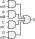
\includegraphics[scale=0.8]{img/enable4bits.pdf}
        \end{center}
        \small
        Las señales \texttt{enA}, \texttt{enB}, \texttt{enC} y \texttt{enD} son de habilitación, para los datos de las señales \texttt{A}, \texttt{B}, \texttt{C} y \texttt{D}.
        \end{block}
    }
    \end{textblock}
\end{frame}

\begin{frame}[fragile]
    \frametitle{Bibliografía}
    \begin{itemize}
     \setlength\itemsep{0.5cm}
    \item[-] \small Tanenbaum, “Organización de Computadoras. Un Enfoque Estructurado”, 4ta Edición, 2000.\\
    \begin{itemize}
     \item \textbf{Capítulo 3 - El nivel de lógica digital} - Páginas 117-127
    \end{itemize}
    \item[-] \small Null, “Essentials of Computer Organization and Architecture”, 5th Edition, 2018.\\
    \begin{itemize}
     \item \textbf{Chapter 3 - Boolean Algebra and Digital Logic:}
     \begin{itemize}
     \item 3.2 - Boolean Algebra
     \item 3.3 - Logic Gates
     \end{itemize}
    \end{itemize}
%     \item[-] \small Silberschatz, “Fundamentos de Sistemas Operativos”, 7ma Edición, 2006.\\
%     \item[-] \small Tanenbaum, “Modern Operating Systems”, 4th Edition, 2015.\\
    \end{itemize}
\end{frame}

\begin{frame}[fragile]
    \frametitle{Ejercicios}
    Con lo visto, ya pueden resolver los primeros tres ejercicios de la Guía de Lógica Digital.
\end{frame}

\begin{frame}[plain]
    \begin{center}
    \vspace{2cm}
    \huge ¡Gracias!\\
    \vspace{2cm}
%     \normalsize Recuerden leer los comentarios adjuntos\\ en cada clase por aclaraciones.
    \end{center}
\end{frame}

\end{document}
